%% 
%% Copyright 2007, 2008, 2009 Elsevier Ltd
%% 
%% This file is part of the 'Elsarticle Bundle'.
%% ---------------------------------------------
%% 
%% It may be distributed under the conditions of the LaTeX Project Public
%% License, either version 1.2 of this license or (at your option) any
%% later version.  The latest version of this license is in
%%    http://www.latex-project.org/lppl.txt
%% and version 1.2 or later is part of all distributions of LaTeX
%% version 1999/12/01 or later.
%% 
%% The list of all files belonging to the 'Elsarticle Bundle' is
%% given in the file `manifest.txt'.
%% 

%% Template article for Elsevier's document class `elsarticle'
%% with numbered style bibliographic references
%% SP 2008/03/01

\documentclass[preprint,12pt, a4paper]{elsarticle}

%% Use the option review to obtain double line spacing
%% \documentclass[authoryear,preprint,review,12pt]{elsarticle}

%% For including figures, graphicx.sty has been loaded in
%% elsarticle.cls. If you prefer to use the old commands
%% please give \usepackage{epsfig}

%% The amssymb package provides various useful mathematical symbols
\usepackage{amssymb}
%% The amsthm package provides extended theorem environments
%% \usepackage{amsthm}

%% The lineno packages adds line numbers. Start line numbering with
%% \begin{linenumbers}, end it with \end{linenumbers}. Or switch it on
%% for the whole article with \linenumbers.
\usepackage{lineno}

\usepackage{float}
\restylefloat{table}

\usepackage{hyperref}

\journal{SoftwareX}

\begin{document}

\begin{frontmatter}

%% Title, authors and addresses

%% use the tnoteref command within \title for footnotes;
%% use the tnotetext command for theassociated footnote;
%% use the fnref command within \author or \address for footnotes;
%% use the fntext command for theassociated footnote;
%% use the corref command within \author for corresponding author footnotes;
%% use the cortext command for theassociated footnote;
%% use the ead command for the email address,
%% and the form \ead[url] for the home page:
%% \title{Title\tnoteref{label1}}
%% \tnotetext[label1]{}
%% \author{Name\corref{cor1}\fnref{label2}}
%% \ead{email address}
%% \ead[url]{home page}
%% \fntext[label2]{}
%% \cortext[cor1]{}
%% \address{Address\fnref{label3}}
%% \fntext[label3]{}

\title{RadLib: a radiative heat transfer model library for CFD}

%% use optional labels to link authors explicitly to addresses:
%% \author[label1,label2]{}
%% \address[label1]{}
%% \address[label2]{}

%\renewcommand{\thefootnote}{\fnsymbol{footnote}}
\author{Victoria B. Stephens}
\author{Sally Jensen}
\author{Isaac Wheeler}
\author{David O. Lignell\corref{cor1}}

\cortext[cor1]{Corresponding author. \ead{davidlignell@byu.edu}}

\address{Department of Chemical Engineering, Brigham Young University, Provo, UT 84602, United States}

\begin{abstract}
%% Text of abstract 
Ca. 100 words
\end{abstract}

\begin{keyword}
%% keywords here, in the form: keyword \sep keyword
radiative heat transfer \sep reacting flows  \sep CFD
\end{keyword}

\end{frontmatter}

\begin{table}[H]
\begin{tabular}{|l|p{6.5cm}|p{6.5cm}|}
\hline
\textbf{Nr.} & \textbf{Code metadata description} & \textbf{Metadata} \\
\hline
C1 & Current code version & TODO 2.1 \\
\hline
C2 & Permanent link to code/repository used for this code version & $github.com/BYUignite/radlib$ \\
\hline
C3 & Code Ocean compute capsule & (in review) \\
\hline
C4 & Legal Code License   & MIT license (MIT) \\
\hline
C5 & Code versioning system used & Git \\
\hline
C6 & Software code languages, tools, and services used & C++, Python 3 \\
\hline
C7 & Compilation requirements, operating environments \& dependencies & CMake, C++, Python 3, Cython \\
\hline
C8 & If available Link to developer documentation/manual & TODO \\
\hline
C9 & Support email for questions & davidlignell@byu.edu \\
\hline
\end{tabular}
\caption{Code metadata.}
\label{} 
\end{table}


\linenumbers

% TO DO
% - update README
% - tag software version
% - decide on and generate documentation

%%%%%%%%%%%%%%%%%%%%%%%%%%%%%%%%%%%%%%%%%%%%%%%%%%%%%%%%%%%%%%%%%%%%%%%%%%%%%%%%

\section{Motivation and significance}
\label{s:motivation}

Modeling radiative heat transfer, and particular radiation absorption coefficients, for CFD is complex and challenging. More specifically, combustion simulations, which can require many complex property models already, are often complicated by the need for accurate radiation modeling, which can be difficult to implement and computationally expensive relative to simulation cost. This can lead to simulations that use oversimplified radiation models, but in cases where radiation is significant relative to the other physical phenomena, oversimplified models can negatively impact the accuracy of simulation results. In some cases, radiative gains or losses are small compared to other sources, sinks, or modes of heat transfer, and radiation can be safely neglected, but many practical engineering systems do not allow this. For example, simple jet flames demonstrate both possibilities: early in a flame's development, turbulent mixing typically dominates heat transfer and dictates flame behavior; late-stage flame phenomena like soot behavior and flame sheet breakthrough, however, increasingly depend on the magnitude of radiative heat losses and are difficult to simulate accurately without a robust radiation model. These problems motivated development of the RadLib library, which provides a framework and uniform interface for radiation property models and implements three powerful models in C++ and Python, giving researchers easier and more convenient access to advanced radiation property models and a consistent framework for further model development. 

The core mechanisms of radiative phenomena are physically and mathematically complex. Unlike other modes of heat transfer, radiation is governed by a set of integro-differential equations that depend on both direction and wavelength, known as the radiative transfer equations (RTE). Solving the RTE for a given system also requires information about the radiative properties of the materials and media involved, typically radiation absorption coefficients. Depending on the model, absorption coefficients can be dependent on a number of local system properties such as temperature, pressure, and gas composition. As a result, computational radiation solvers require two parts: first, a solution approach for the radiative transfer equations (RTE); and second, a radiation property model. RadLib addresses the second part by providing a set of implemented and validated radiation property models that can be applied to various solution approaches for the RTE. 

%Like combustion, the core mechanisms of radiation are physically and mathematically complex. Unlike other modes of heat transfer, radiation is governed by a set of integro-differential equations that depend on both direction and wavelength. Only the simplest systems have analytic solutions, and most practical systems require a numerical solution. Ray tracing solutions are very accurate but extremely computationally expensive, and often require high-performance computing resources to execute. Modeling assumptions are common and can reduce simulation cost at the expense of accuracy, depending on their validity for the system in question. 

With RadLib, we provide a convenient, easy-to-use access point for radiative property models that can be interfaced with various RTE solution approaches suitable for CFD applications. RadLib is a modular C++ library with an optional Python interface used to compute the radiation properties of participating media, often the most difficult and time-consuming portion of radiation calculations. RadLib's current focus is calculating radiation absorption coefficients and weighting factors for use in global radiation models, but the flexible framework permits expansion to other radiative properties. Three models are fully implemented and validated and all use a common interface, allowing researchers easy and convenient access to radiation modeling tools regardless of the field of application.

%%%%%%%%%%%%%%%%%%%%%%%%%%%%%%%%%%%%%%%%%%%%%%%%%%%%%%%%%%%%%%%%%%%%%%%%%%%%%%%%

\section{Model descriptions}
\label{s:models}

To give context to the following discussion of radiative individual property models, we include here a brief description of the radiative transfer equation (RTE). Along a given path length $s$ in a direction $\hat{\Omega}$, the general RTE  for an absorbing, emitting, and non-scattering medium is described by 
\begin{equation}
	\label{e:RTE_general}
	\frac{dI_{\eta}}{ds} = -\kappa_{\eta}I_{\eta} + \kappa_{\eta}I_{b \eta},
\end{equation}
where $I_{\eta}$ is the radiative spectral intensity, $I_{b\eta}$ is the Planck spectral distribution of blackbody intensity, and $\kappa_{\eta}$ is the spectral absorption coefficient of the medium. Radiation property models such as those implemented by RadLib are used to calculate the absorption coefficients $\kappa_{\eta}$. From this point, various approximations can be made to simplify the solution process. For example, integrating with respect to wavenumber and subdividing the absorption cross-section into gray gases gives the spectral line-weighted (SLW) form of the RTE,
\begin{equation}
\label{e:RTE_SLW}
	\frac{dI_j}{ds} = -\kappa_jI_j + a_j\kappa_jI_b, \hspace{20pt} j=0,1,...,n,
\end{equation}
where $n$ is the number of gray gases in the model, $I_j$ is the intensity of gray gas $j$, and $\kappa_j$ represents the gray gas absorption coefficient for gas $j$. When multiple gray gases are used to approximate the radiative properties, the total radiative intensity $I$ can be calculated by summing the individual gray gas intensities calculated with Equation \ref{e:RTE_SLW}:
\begin{equation}
	I=\int_{\eta=0}^{\infty}I_{\eta}d\eta=\sum_{j=1}^n I_j.
\end{equation}
From there, the total radiative intensity can be used to calculate various radiative heat fluxes and, where appropriate, be incorporated into larger energy balances for a simulation.

RadLib implements three models of varying complexity and accuracy to calculate the radiation absorption coefficients $\kappa$ and their weighting factors $a$ for each gas considered by the model. The absorption coefficients are typically calculated using correlations relating them local properties such as temperature, pressure, and composition. Correlations come from curve fits to high-resolution radiation property databases. At present, RadLib considers up to four gas species (H$_2$O, CO, CO$_2$, and CH$_4$) and soot in its calculation of absorption coefficients and weighting factors. 

Once the radiative absorption coefficients are calculated, they can then be used to solve the RTE, which depends on the simulation configuration and assumptions. Solving the RTE is not the focus of this software, but RadLib's example cases do employ a simple ray tracing solver to calculate the radiative heat flux and volumetric heat source profiles between two parallel planes. 

%[OTHER THINGS THAT APPLY TO ALL MODELS GO HERE]

\subsection{Planck Mean absorption coefficients}
\label{s:planckmean}

RadLib's simplest model uses Planck Mean absorption coefficients calculated from the correlations given on the TNF Workshop site \citep{Smith_2003}. The temperature-dependent correlations are based on the RADCAL model in \citep{Grosshandler_1993}. The TNF radiation model is also documented in \citep{Barlow_2001}.

Planck Mean absorption coefficients are commonly used to model radiation, especially in combustion systems, because the model is relatively easy to implement, computationally inexpensive, and reasonably accurate in some cases. The Planck Mean model is most appropriate under optically thin conditions with relatively low radiative transfer relative to other heat sources such as reactive heat release rates. In cases where the optically thin assumption applies, such as simple hydrogen jet flames, this model and the associated Planck Mean absorption coefficients can produce accurate results \citep{Barlow_1999}. In cases where the optically thin assumption is not reasonable, including many other combustion scenarios, the Planck Mean model does not produce accurate results. For example, it significantly overpredicts radiative losses from the TNF library's CH$_4$ flames \cite{Frank_2000,Zhu_2002,Coelho_2002}. The examples included with the code and illustrated in Section \ref{s:Examples} demonstrate the deficiencies of the Planck Mean model in comparison to the others included with RadLib.

\subsection{Weighted sum of gray gases (WSGG)}
\label{s:wsgg}
The basic assumption of weighted sum of gray gases (WSGG) models in general is that the non-gray behavior of gas mixtures, in this case H$_2$O and CO$_2$, can be modeled by a weighted sum of several gray gases and one transparent gas (which represents the spectral windows between absorption bands). 
RadLib implements the WSGG model presented by Bordbar et al. \citep{Bordbar_2014,Bordbar_2020}, which uses correlations based on the HITEMP 2010 database \cite{Rothman_2010}. It uses four gray gases and one transparent gas. Absorption coefficients are calculated by 
\begin{equation}
 K_i=\sum_{k=0}^{4}d_{i,k}M_r^k,
\end{equation}
where $K_i$ is the absorption coefficient for species $i$, $d_{i,k}$ is a species-specific correlated model coefficient, and $M_r$ is the molar ratio $Y_{\mathrm{H_2O}}/Y_{\mathrm{CO_2}}$. The weight factors are calculated by 
\begin{equation}
 a_i=\sum_{j=0}^{4}b_{i,j}T_r^j,
\end{equation}
where $a_i$ is the weighting factor for species $i$ and $T_r$ is a normalized temperature equal to $T/T_{ref}$ with $T_{ref}=1200$K. The value of $b_{i,j}$ is calculated by 
\begin{equation}
 b_{i,j}=\sum_{k=0}^{4}C_{i,j}M_r^k,
\end{equation}
where $C_{i,j}$ is another correlated model coefficient and $M_r$ is the molar ratio $Y_{\mathrm{H_2O}}/Y_{\mathrm{CO_2}}$ as above. The model coefficients $d_{i,k}$ and $C_{i,j}$ can be found in the literature \citep{Bordbar_2014,Bordbar_2020}. 

Previous WSGG versions and other property models often considered weighting factors as a function of temperature only and assumed a fixed molar ratio of H$_2$O and CO$_2$. This version includes dependence on both temperature and an arbitrary molar fraction ratio, increasing its accuracy and flexibility. RadLib uses the updated model coefficients from \citep{Bordbar_2020}, which extends the limited range of H$_2$O-CO$_2$ molar ratios originally presented in \citep{Bordbar_2014}. 


\subsection{Rank Correlated SLW (RCSLW)}
\label{s:RCSLW}

The Spectral Line Weighted-sum-of-gray gases (SLW) model represents a family of global approaches to radiative heat transfer in high-temperature gases that also includes Absorption Distribution Function (ADF) and Full Spectrum $k$-distribution (FSK) models, all of which are based on the same fundamental principle in modeling the gas absorption spectrum \cite{Solovjov_2016}. In order to extend their spectral models from uniform conditions (isothermal, homogeneous gases) to nonuniform conditions (non-isothermal, non-homogeneous gases), these models take a reference approach in which local gas states are corrected relative to a reference state. Reference approaches, however, generally lack consistent reference states and can yield significant errors in cases with large spatial temperature gradients \cite{Solovjov_2017}. The Rank Correlated SLW (RCSLW) model is a unique extension of the generalized SLW model that does not require a specified gas reference state and preserves the emission term of the spectrally integrated RTE. Recent comparison of advanced SLW modeling approaches revealed that "the Rank Correlated SLW model is the most robust of all models, and demonstrates that it can achieve accurate solutions with as few as 3–5 gray gases" \citep{Badger_2019}. A brief overview of the general SLW and RCSLW models will be given here; detailed discussion can be found in the literature \cite{Solovjov_2000, Solovjov_2001, Solovjov_2008, Solovjov_2011, Solovjov_2014, Solovjov_2016, Solovjov_2017, Webb_2018}. 

The RCSLW model begins with the SLW form of the RTE, given by Equation \ref{e:RTE_SLW}. The gray gas absorption coefficients $\kappa_j$ are calculated calculated as $\kappa_j=N \sqrt{C_{j-1}C_j}$,
where $C_{j-1}$ and $C_j$ are supplemental absorption cross-sections used to discretize the absorption spectrum \cite{Solovjov_2001}. The gray gas weights $a_j$ corresponding to each absorption coefficient are given by $a_j=F(C_j)-F(C_{j-1})$, where $F(C_j)$ is the absorption line blackbody distribution function (ALBDF) for species $j$, calculated from the detailed absorption spectrum of that species. In general SLW methods, the absorption cross-sections are chosen with respect to a thermodynamic reference state, classifying them as reference approaches. The Rank-Correlated SLW (RCSLW) model avoids specifying a reference state by relating thermodynamic states to one another instead. If two arbitrary absorption cross-sections define identical wavenumber intervals, the two cross-sections (neither of which is designated a reference cross-section) can be said to be rank-correlated. The inverse ALBDF, defined such that $C[F(C,\phi_g,T_b),\phi_g,T_b]=C$ and $F[C(F,\phi_g,T_b),\phi_g,T_b]=F$ for a given gas thermodynamic state $\phi_g$ and blackbody temperature $T_b$, is proven to have this property and can also be called the rank-correlated reordered absorption cross-sections \cite{Solovjov_2017}. As a result, the inverse ALBDF can be used to construct cross-section intervals for the RCSLW model that do not rely on an arbitrary reference state or spectrum. RadLib's RCSLW model uses Method 1.2.2 as defined and recommended in \cite{Solovjov_2017}.

%%%%%%%%%%%%%%%%%%%%%%%%%%%%%%%%%%%%%%%%%%%%%%%%%%%%%%%%%%%%%%%%%%%%%%%%%%%%%%%%

\section{Software Description}
\label{s:architechture}

RadLib is an object-oriented C++ class library that includes both C++ and Python interfaces. The RadLib package contains five subdirectories (upon initial download): \texttt{source} contains the RadLib source code; \texttt{build} contains installation files; \texttt{examples} contains instructive example cases, including a simple interface and solver for a parallel planes geometry; \texttt{data} contains ALBDF data tables required for the RCSLW model; and \texttt{docs} contains files used to generate code documentation with Doxygen (optional). 

The \texttt{source} and \texttt{examples} directories are further divided into \texttt{C++} and \texttt{Python} subdirectories to differentiate between interfaces. There are three interface options for using this code: C++, Python, and Cython-wrapped Python. C++ interfaces are located within the \texttt{examples/c++} folder, while Python interfaces are located within the \texttt{examples/python} folder. When running examples with Python, the Cython-wrapped version is the default; to run the regular Python version without the Cython wrapper, edit the comments near the top of the example files (i.e \texttt{ex\textunderscore S1.py}). The C++ interface produces the fastest-running code, followed by the Cython-wrapped Python interface and then the regular Python interface. [INSERT RUNTIME COMPARISONS HERE]

RadLib installation is automated with CMake. First, navigate to the \texttt{radlib/build} directory. If the user requires an installation location other than the default \texttt{radlib/installed} directory, edit the \texttt{user\textunderscore config} file before running CMake. To compile the package, run the command \texttt{cmake -C user\textunderscore config ../source}. Upon successful completion, run \texttt{make} and then \texttt{make install} to complete the process. The generated C++ library file is located at \texttt{radlib/installled/lib/libradlib.a}. 

Figure \ref{fig:flowchart} illustrates the basic structure use of the RadLib package within a generic example using the provided interfaces. The RadLib library generates absorption coefficients and their weighting factors for use within the appropriate RTE, but does not specify any particular geometry, making it a versatile tool for any simulation that requires radiative heat transfer, regardless of configuration. The interfaces, solver, and examples included with the library serve to illustrate its use and validate the implementation and results. 

\begin{figure}
	\begin{center}
		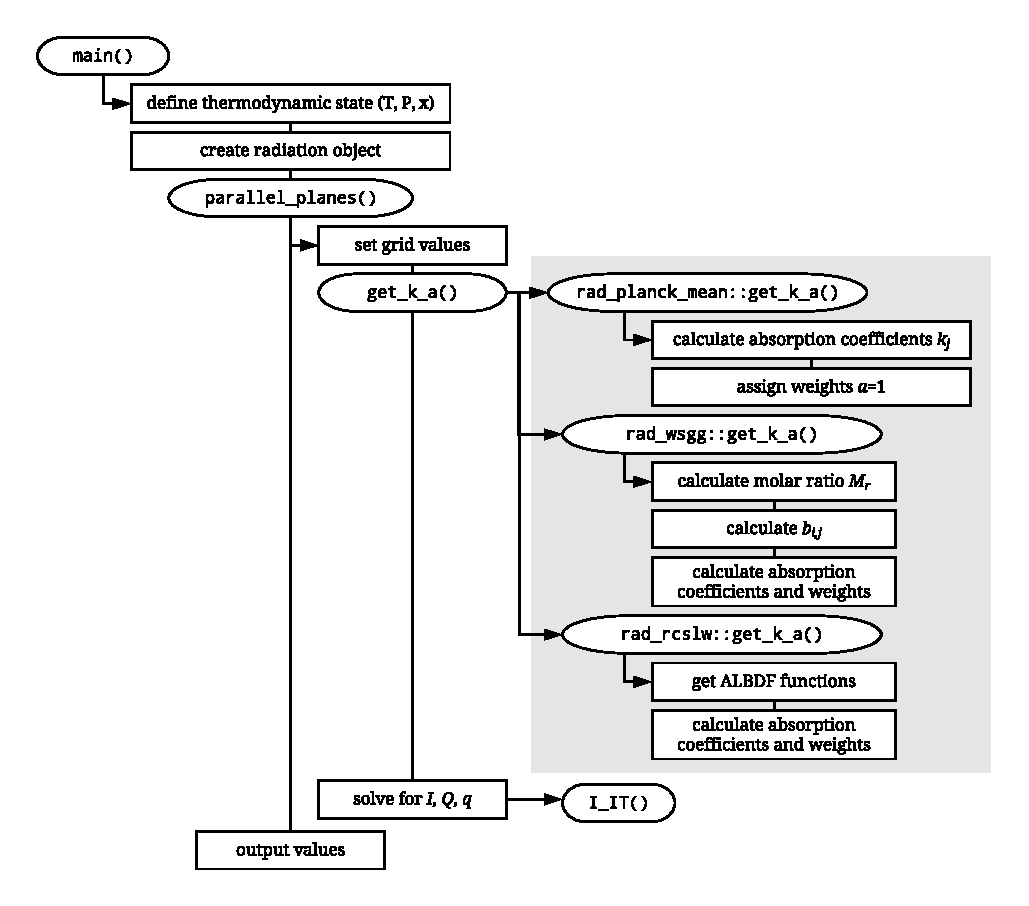
\includegraphics[width=\textwidth]{../figures/radlib_structure.pdf}
	\end{center}
	\caption{Example workflow diagram. Highlighted areas are part of the RadLib library; other areas represent example infrastructure for using the package.}
\label{fig:flowchart}
\end{figure}

%%%%%%%%%%%%%%%%%%%%%%%%%%%%%%%%%%%%%%%%%%%%%%%%%%%%%%%%%%%%%%%%%%%%%%%%%%%%%%%%

\section{Illustrative Examples}
\label{s:Examples}

Several examples are presented to illustrate the behavior of the models. The examples show heat flux $q$ or volumetric heat source $Q$ in one one-dimensional configurations with varying gas compositions and temperatures. We compare the PM, WSGG, and RCSLW models for each example. The examples correspond to those presented by Solvojov et al. (S) \cite{Solovjov_2017} and Bordbar et al. (B) \cite{Bordbar_2020}, and the number of each example corresponds to the example number in the respective reference. A ray-tracing code is used to solve the radiative transport equation between two parallel plates. 
Table~\ref{t:examples} summarizes the cases. Example S1 is a hot slab next to a cold slab where the cold slab's thickness varies; Example S2 is isothermal with a thick slab of high CO$_2$ next to a thin slab of low CO$_2$ with variable thickness; Example S3 uses parabolic temperature and H$_2$O mole fraction profiles; Example S4 has a triangular temperature profile between equally-spaced isothermal regions; Example S5 uses a half-sinusoid temperature profile that decreases from 1500 to 500 K; and Example B3 has symmetric temperature and H$_2$O mole fraction profiles with central peaks of 1800 K and 1, respectively (with $y_{CO2}=1-y_{H2O}$). Each case is presented alongside the line-by-line (LBL) data presented in the references. 
%
\begin{table}
    \caption{Summary of example cases presented. S1-S5 are from \cite{Solovjov_2017}; B3 is from \cite{Bordbar_2020}. All cases use $P=1$ atm and black walls.}
    \label{t:examples}
    \centering
    \resizebox{\textwidth}{!}{
    \begin{tabular}{c l l c c c}
        \hline
        Example & T(K)                           & $y_{H2O}$  $y_{CO2}$ (mole frac.)                     & L (m)   & $T_{walls}$ (K)\\
        \hline
        S1 & $T(x<0.5)=2000$; $T(x>0.5)=300$     & $y_{CO2}=0.1$, $y_{H2O}=0.2$                          & 0.5-2.5 & cold, cold     \\
        S2 & T=1000                              & $y_{CO2}(x<0.5)=0.4$, $y_{CO2}(x>0.5)=0.1$            & 0.5-2.5 & cold, cold     \\
           &                                     & $y_{H2O}=0.0$                                         &         &                \\
        S3 & $T(x) = 4000x(L-x)/L^2 + 800$       & $y_{H2O}(x) = 0.8x(L-x)/L^2 + 0.12$                   & 1       & 800, 800       \\
           &                                     & $y_{CO2}=0$                                           &         &                \\
        S4 & middle third triangular to 2500     & $y_{H2O}=0.1$, $y_{CO2}=0$                            & 0.3     & 500, 500       \\
        S5 & $T(x) = 1000 + 500\cos(\pi x/L)$    & $y_{H2O}=0.1$, $y_{CO2}=0$                            & 2       & 1500, 500      \\
        B3 & $T(x) = 400 + 1400\sin(\pi x/L)^2$  & $y_{H2O}(x) = 0.0001 + 0.9999\sin(\pi x/L)^2$         & 1       & 400, 400       \\
           &                                     & $y_{CO2}=1-y_{H2O}$                                   &         &                \\
        \hline
    \end{tabular}
    }
\end{table}
%

The examples are provided with the RadLib code and implemented in both C++ and Python. A Juptyer notebook is provided with the Python examples that runs the examples, displays the plots, and saves the plots to PDF files. Python and Cython versions of the one-dimensional solver \texttt{parallel\textunderscore planes.py} are provided for convenience. 

These cases are intended to illustrate the use of the RadLib library and are not exhaustive. Details about these examples and their motivations can be found in their respective references. While ommitted here for brevity, the implemented WSGG and RCSLW models give essentially identical results to those presented in \cite{Solovjov_2017,Bordbar_2020} such that these examples also serve as a validation of the implementation of the models.

Figure~\ref{f:examples} shows comparative results for the different radiation models for these cases. 
%
\begin{figure}
    \begin{center}
    \begin{tabular}{c c}
        Example S1 & Example S2 \\
        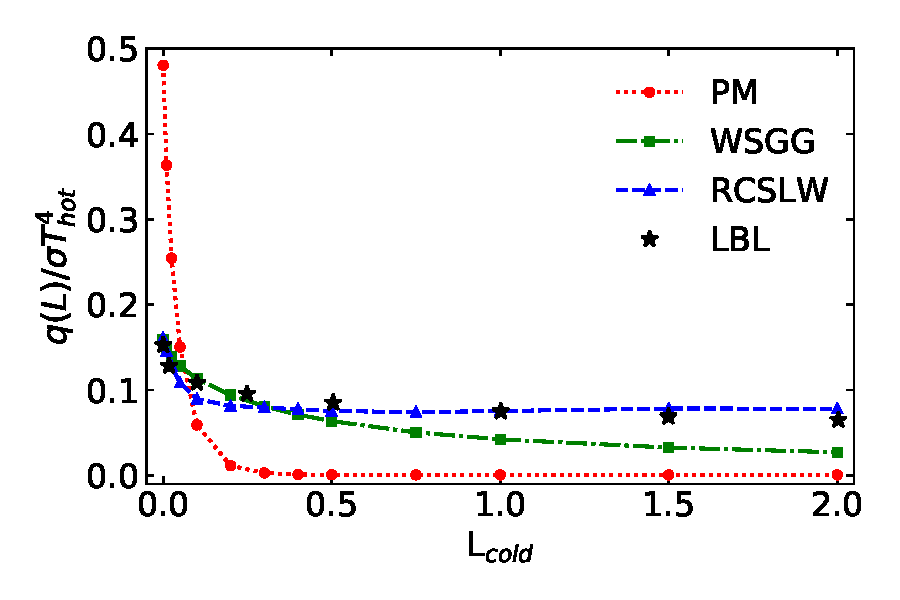
\includegraphics[width=3 in]{ex_1.pdf} &
        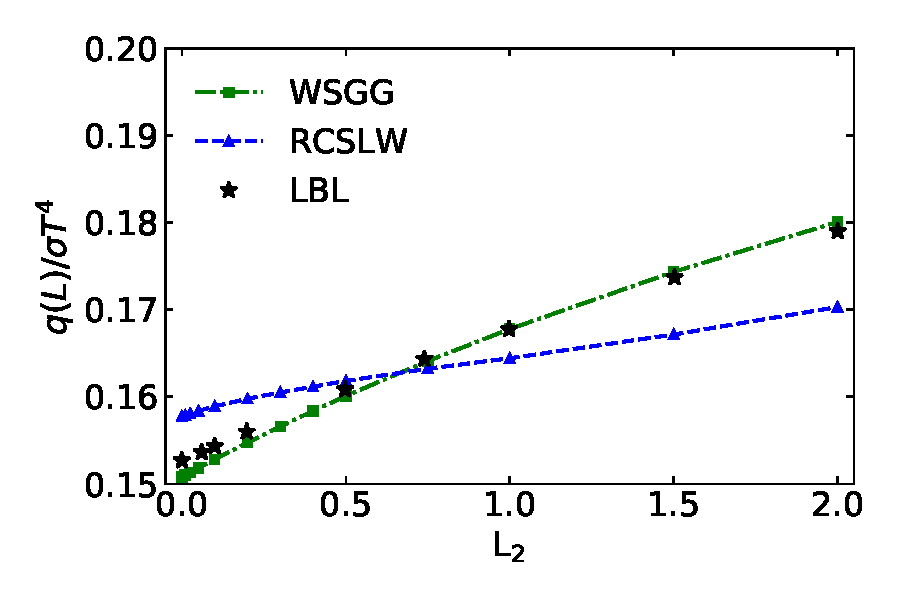
\includegraphics[width=3 in]{ex_2b.pdf} \\
        Example S3 & Example S4 \\
        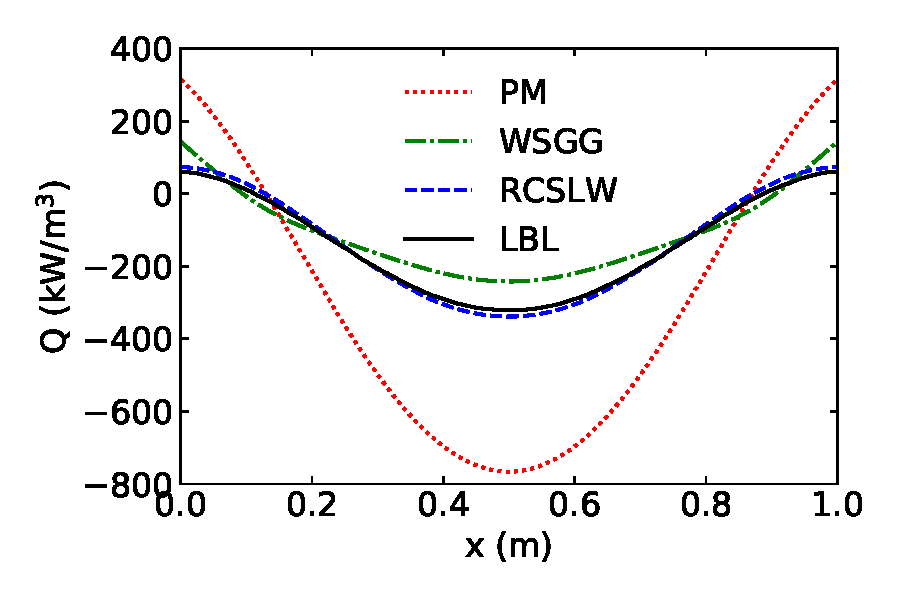
\includegraphics[width=3 in]{ex_3a.pdf} &
        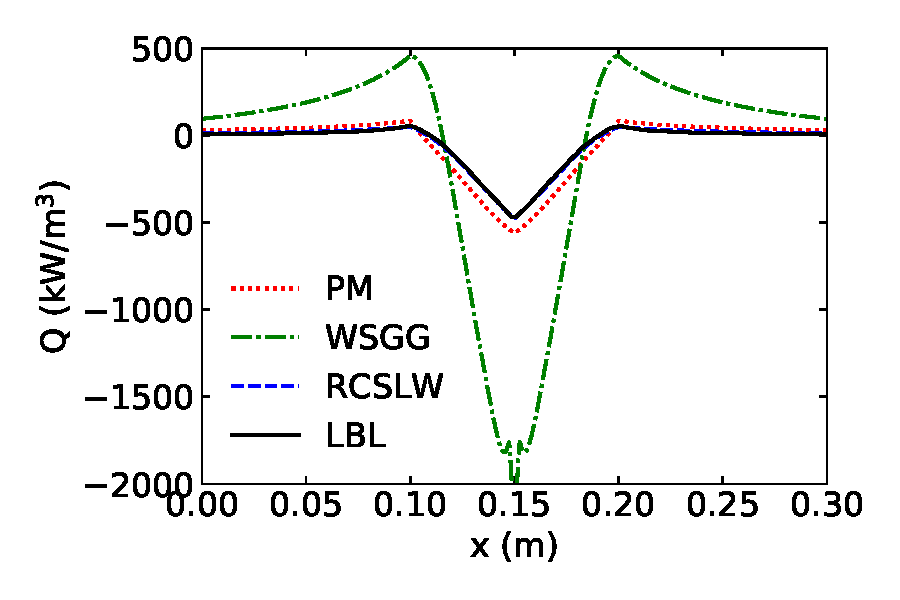
\includegraphics[width=3 in]{ex_4a.pdf} \\
        Example S5 & Example B3 \\
        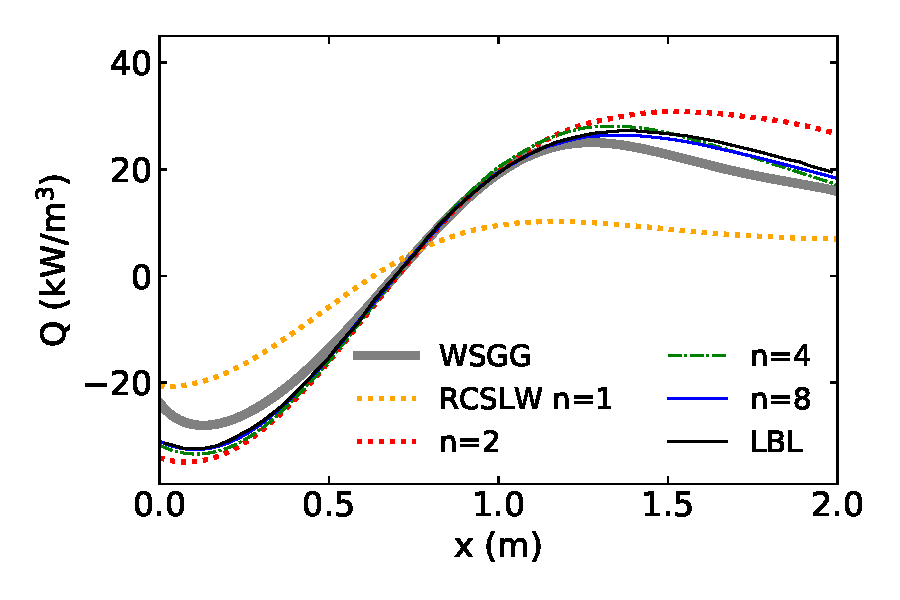
\includegraphics[width=3 in]{ex_5b.pdf} &
        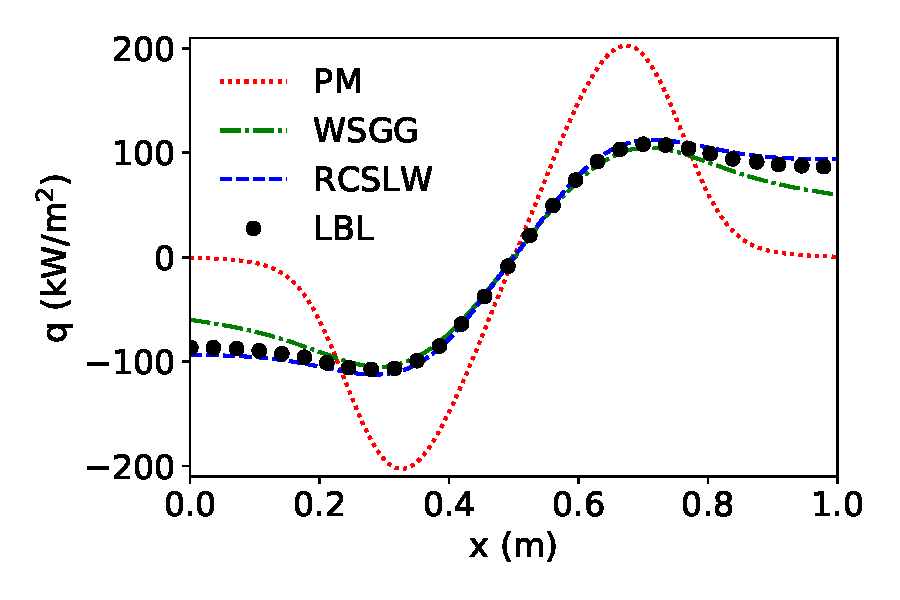
\includegraphics[width=3 in]{ex_6.pdf}
    \end{tabular}
    \caption{Results for examples summarized in Table~\ref{t:examples}.}
    \label{f:examples}
    \end{center}
\end{figure}
%
In general, the PM model performs poorly compared to the WSSGG and RCSLW models. A notable exception is Example S4. In Example S2, the PM $q(L)/\sigma T^4$ is off scale at an essentially constant at a value of unity. The PM absorption coefficient is 27.4 atm$^{-1}$m$^{-1}$, giving optical thicknesses of 0.09 and 0.36 m in the thick and thin layers, respectively, which are relatively small compared to the isothermal domain size greater than 0.5 m. Example S5 omits the PM model to more clearly show the behavior of the WSGG and RCSLW models. For that example, the PM values follow the shape of the other curves but $Q$ varies from around -80 at $x=0$ to a peak of 200 at x=$1.5$ m, and dropping to 100 kW/m$^3$ at $x=2$ m. In all examples, four gray ($n=4$) and one clear gas are computed for the RCSLW models to give a consistent comparison to the WSGG model. Example S5 shows the sensitivity of the RCSLW model to the number of gases used. When $n$ is increased to eight the RCSLW model improves to show nearly perfect agreement with the LBL data in Example S2.
In all Examples, the RCSLW model is initialized using the mean temperature and composition on the domain. In Example S5, the RCSLW model converges to the LBL solution when the model is initialized using the maximum temperature instead of the average temperature.

% TODO: do the cost comparison  <13-11-20, dol> %

%%%%%%%%%%%%%%%%%%%%%%%%%%%%%%%%%%%%%%%%%%%%%%%%%%%%%%%%%%%%%%%%%%%%%%%%%%%%%%%%

\section{Impact}
\label{s:impact}

Radiative heat transfer models are historically difficult to implement in CFD codes due to their complexity and high computational costs. Neglecting radiation or using simple models like the optically thin assumption is adequate for some cases with simple geometry or limited chemical reactions, but most simulations of interest to engineers and researchers require more advanced radiation modeling to yield accurate results. In such cases, radiation models that are incorrectly implemented or inappropriate for the simulation parameters can become additional sources of error that may be extremely difficult to separate from existing sources or error. Currently, researchers that require detailed radiation modeling must code and validate it themselves at the expense of valuable research time and funding. 

RadLib makes researchers' work easier by consolidating various approaches into a modular library of interchangeable, prevalidated radiation models. Additionally, RadLib's modular framework is designed to easily accommodate new models as well, allowing researchers to compare new or existing models with very little overhead. Sometimes, it is not clear which radiation model may be the best fit for a particular simulation. When simulations are especially complex or computationally expensive, researchers may have to extrapolate from theory and literature to choose an appropriate radiation model rather than testing for their specific case. RadLib is designed to ease both of these obstacles by facilitating comparison between radiation models through a common interface and providing a practical means of testing various models without the restriction of prespecified geometry or case parameters. With RadLib, researchers can put more of their time and effort into useful results rather than code or model development. 

Currently, RadLib is only used within the authors' research group, where it is applied to combustion CFD simulations using the One-Dimensional Turbulence (ODT) model \cite{Stephens_2020}, but its design and structure as a C++ library allows it to be incorporated easily into existing codes. It can be applied to  research questions in various other fields involving radiative heat transfer as well, including energy engineering or atmospheric and climate sciences. Radiation is a universal phenomenon, and RadLib can assist researchers in many areas with systems and processes that involve heat transfer. 

%Author guidelines for this section
%\begin{itemize}
% \item \textbf{This is the main section of the article and the reviewers weight the description here appropriately}
% \item Indicate in what way new research questions can be pursued as a result of the software (if any).
% \item Indicate in what way, and to what extent, the pursuit of existing research questions is improved (if so).
% \item Indicate in what way the software has changed the daily practice of its users (if so).
% \item Indicate how widespread the use of the software is within and outside the intended user group.
% \item Indicate in what way the software is used in commercial settings and/or how it led to the creation of spin-off companies (if so).
%\end{itemize}

%%%%%%%%%%%%%%%%%%%%%%%%%%%%%%%%%%%%%%%%%%%%%%%%%%%%%%%%%%%%%%%%%%%%%%%%%%%%%%%%

\section{Conclusions}
\label{}

Set out the conclusion of this original software publication.

%%%%%%%%%%%%%%%%%%%%%%%%%%%%%%%%%%%%%%%%%%%%%%%%%%%%%%%%%%%%%%%%%%%%%%%%%%%%%%%%

\section{Conflict of Interest}

There are no known conflicts of interest associated with this publication and there has been no significant financial support for     this work that could have influenced its outcome.

%%%%%%%%%%%%%%%%%%%%%%%%%%%%%%%%%%%%%%%%%%%%%%%%%%%%%%%%%%%%%%%%%%%%%%%%%%%%%%%%

\section*{Acknowledgements}
\label{sec:acknowledgements}

The authors extend special thanks to Hadi Bordbar for assistance with the WSGG model and to Vladimir Solovjov and Brent Webb of Brigham Young University for their insights and assistance with the RCSLW model. 

%%%%%%%%%%%%%%%%%%%%%%%%%%%%%%%%%%%%%%%%%%%%%%%%%%%%%%%%%%%%%%%%%%%%%%%%%%%%%%%%

%% \appendix

%% \section{}
%% \label{}

%%%%%%%%%%%%%%%%%%%%%%%%%%%%%%%%%%%%%%%%%%%%%%%%%%%%%%%%%%%%%%%%%%%%%%%%%%%%%%%%
%% References:

\bibliographystyle{elsarticle-num} 
\bibliography{references} 

%%%%%%%%%%%%%%%%%%%%%%%%%%%%%%%%%%%%%%%%%%%%%%%%%%%%%%%%%%%%%%%%%%%%%%%%%%%%%%%%

\section*{Current executable software version}
\label{}

%Ancillary data table required for sub version of the executable software: (x.1, x.2 etc.) kindly replace examples in right column with the correct information about your executables, and leave the left column as it is.

\begin{table}[!h]
\begin{tabular}{|l|p{6.5cm}|p{6.5cm}|}
\hline
\textbf{Nr.} & \textbf{(Executable) software metadata description} & \textbf{Metadata} \\
\hline
S1 & Current software version & 1.0 \\
\hline
S2 & Permanent link to executables of this version  & \href{https://github.com/BYUignite/radlib}{https://github.com/BYUignite/radlib} \\
\hline
S3 & Legal Software License & MIT license (MIT) \\
\hline
S4 & Computing platforms/Operating Systems & Linux, OS X, Microsoft Windows\\
\hline
S5 & Installation requirements \& dependencies & CMake, C++, Python 3, Cython \\
\hline
S6 & If available, link to user manual - if formally published include a reference to the publication in the reference
    list & \href{https://github.com/BYUignite/radlib}{https://github.com/BYUignite/radlib} \\
\hline
S7 & Support email for questions & davidlignell@byu.edu \\
\hline
\end{tabular}
\caption{Software metadata.}
\label{} 
\end{table}

\end{document}
\endinput
